\section{ AR0030IR18 }


\subsection{Meta}

    \textbf{Title:}
    A state of the art review of intelligent scheduling

    \begin{table}[H]
        \centering
        \begin{tabular}{|c|c|c|c|c|c|c|c|c|c|}
            \hline
                \textbf{Rel} & \textbf{Grade} & \textbf{Type} & \textbf{Domain} & \textbf{Output}  & \textbf{Grasp}   & \textbf{Gp} & \textbf{COV19} & \textbf{CoI} & \textbf{Fund} \\
            \hline
             - & - & - & - & - & - & - & - & - & - \\
            \hline
        \end{tabular}
        \caption{Reference's metadata}
        \label{tab:AR0030IR18}
    \end{table}

\subsection{Summary}
    Mohammad Hossein Fazel Zarandi et al. \cite{032IRSchedulingReview2020} 

\subsection{Notes}
    \begin{itemize}
        \item Metaheuristics Pros and Cons;
        \item Fuzzy logic;
        \item Expert systems;
        \item Machine learning;
        \item Stochastic local search optimization algorithms;
        \item Constraint programming;
    \end{itemize}


\subsection{Reading}
    \textbf{Abstract:}
        The intelligent scheduling is a broad area with numerouse approaches and techniques. The presenter work covers five the most popular methods of intelligent scheduling with implementations of the case studies.
    
    \textbf{Objectives:}
        Not specified.

    
    \textbf{Materials:}
    \begin{figure}[H]
        \centering
        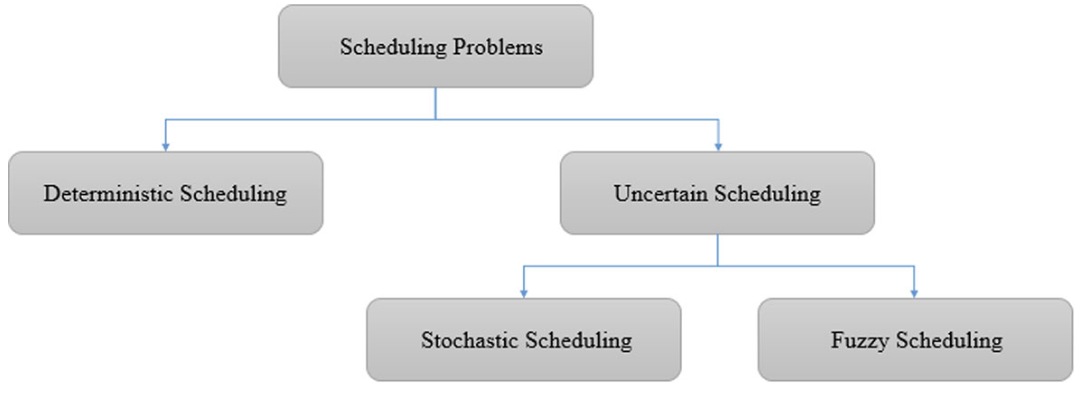
\includegraphics[width=1\textwidth]{figures/AR0030IR18/fig1.png}
        \caption{Classification of the scheduling problem by \cite{032IRSchedulingReview2020}.}
        \label{fig1:AR0030IR18}
    \end{figure}
    